\documentclass[a4paper, 11pt]{scrartcl}

\usepackage[utf8]{inputenc}
\usepackage[ngerman]{babel}

\usepackage{mathptmx}
\renewcommand{\familydefault}{\sfdefault}

% Settings for page geometry
\usepackage[left=2.5cm, right=2.5cm, top=2.5cm, bottom=2.5cm]{geometry}
\usepackage[onehalfspacing]{setspace}

% ETC Packages
\usepackage{amsmath}
\usepackage{amssymb}
\usepackage{graphicx}
\usepackage{xcolor}
\usepackage{floatflt,epsfig}
\usepackage{scrlayer-scrpage}
\usepackage{hyperref}
\usepackage{float}
\usepackage{sectsty}

\usepackage{xcolor}
\usepackage{floatflt,epsfig}
\usepackage[framemethod=tikz]{mdframed}
% \usepackage[fleqn]{amsmath}
\usepackage{listings}
\usepackage{color}
%\usepackage{minted}

\mdfsetup{
    skipabove=\topskip ,
    skipbelow=\topskip ,
    innertopmargin=-0.2cm,
    innerbottommargin=-0.2cm,
    innerleftmargin=0cm
}

\definecolor{dkgreen}{rgb}{0,0.6,0} % comment style
\definecolor{gray}{rgb}{0.5,0.5,0.5}
\definecolor{mauve}{rgb}{0.58,0,0.82} 
\definecolor{BBS}{RGB}{0,169,164} % Teal color of BBS logo
\definecolor{ssh}{RGB}{22,198,12} % bash connection / user
\definecolor{path}{RGB}{59,120,184} % Bash current working directory
\definecolor{bbg}{RGB}{50,50,50} % Bash Background
\definecolor{cfg}{RGB}{58,150,221} % Bash Background

\lstset{ % defining an environment for bash code
    escapeinside={<@}{@>},
    aboveskip=3mm,
    belowskip=3mm,
    showstringspaces=false,
    columns=flexible,
    basicstyle={\small\ttfamily\color{white}},
    numbers=none,
    numberstyle=\tiny\color{white},
    commentstyle=\color{dkgreen},
    stringstyle=\color{blue},
    breaklines=true,
    breakatwhitespace=true,
    tabsize=3,
    morekeywords={
        sudo, apt, git, ufw
    }
}

% Define colors for headings of different parts of the documentation
\sectionfont{\color{BBS}}
\subsectionfont{\color{BBS}}
\subsubsectionfont{\color{BBS}}

\begin{document}
% \begin{spacing}{1.3}
\thispagestyle{empty}
\ihead{
    \begin{footnotesize}
        Deployment einer Rest API
    \end{footnotesize}
}
\chead{
    \begin{footnotesize}
        Lernfeld 9: Netzwerke und Dienste bereitstellen
    \end{footnotesize}
}
\ohead{
    \begin{footnotesize}
        Gerrit Koppe
    \end{footnotesize}
}
\vspace{0.2\textheight}
\begin{center}
    \begin{figure}[H]
        \begin{minipage}{0.3\textwidth}
            
\includegraphics[scale=0.6]{Bilder/BBS}
        \end{minipage}
        \hspace{0.48\textwidth}
        \begin{minipage}{0.3\textwidth}
            
\includegraphics[scale=0.6]{Bilder/sievers.png}
        \end{minipage}
    \end{figure}
    \vspace{1cm}
    \begin{Huge}
        \textcolor{BBS}{\textbf{Dokumentation Deployment einer Rest API}}
    \end{Huge}
    \\
    \vspace{0.1\textheight}
    \begin{Large}
        Autor: Gerrit Koppe
    \end{Large}
    \\
    \vspace{0.5cm}
    \begin{Large}
        Ausbildungsberuf: Fachinformatiker für Anwendungsentwicklung
    \end{Large}
    \\
    \vspace{0.5cm}
    \begin{Large}
        Klasse: IFA12
    \end{Large}
    \\
    \vspace{0.5cm}
    \begin{Large}
        Lernfeld 9: Netzwerke und Dienste bereitstellen
    \end{Large}
    \\
    \vspace{0.5cm}
    \begin{Large}
        \today
    \end{Large}
\end{center}
\newpage
\thispagestyle{empty}
\begin{Large}
    \begin{flushleft}
        \textbf{\textcolor{BBS}{Anmerkungen}}
    \end{flushleft}
\end{Large}
Aus Gründen der Leserlichkeit wird in dieser Dokumentation das Wort \glqq Server\grqq{} verwendet, wann immer vom Raspberry Pi die Rede ist.
\\
Alle ausgeführten Befehle werden im laufenden Text der Dokumentation angegeben. Währed des gesamten Prozesses, welcher in dieser Dokumentation beschrieben wird, wurden des Weiteren Screenshots
gemacht, welche in den Anlagen in Kapitel \ref{ch:pics} beigefügt sind. Auf diese wird an den entsprechenden Stellen der Dokumentation verwiesen.
\\
Wann immer in einer Terminal Abbildung \glqq\lstinline[basicstyle={\small\ttfamily\color{black}}]|#...|\grqq{} steht, zeigt dies an, dass die Datei, welche jeweils bearbeitet wurde,
weitere Zeilen hat, welche aber nicht relevant für den jeweils aktuellen Arbeitsschritt sind und dementsprechend ausgelassen wurden.

\newpage
\thispagestyle{empty}
\tableofcontents
\newpage
\clearpage
\pagenumbering{arabic}


\section{Einleitung}
In dieser Dokumentation wird die Konfiguration eines Raspberry Pi\footnote{Fortan \glqq Server\grqq} als Host einer Rest API, sowie das Deployment besagter Rest API beschrieben.
\\
Es wird zunächst auf allgemeine Vorbereitungen eingegangen. Anschließend wird beschrieben, wie die User und das Netzwerk, sowie die Firewall des Servers konfiguriert werden müssen.
Abschließend wird die Installation des Webservers, sowie das Deployment der Rest API auf dem Server beschrieben.
\\
Sämtliche Arbeitsschritte sind sowohl durch die jeweiligen Terminal Befehle, als auch durch Screenshots die während der Umsetzung entstanden sind, dokumentiert.



\section{Vorbereitungen}
% Inbetriebnahme Raspberry PI
% Betriebssystem, Einbinden in Netzwerk

\section{Konfiguration der User}\label{ch:user}
% Benötigte User und warum
% TODO Begründung anpassen.
Nachdem das Betriebssystem des Servers installiert, der Server in das Netzwerk eingebunden und überprüft wurde, ob eine SSH Verbindung zum Server möglich ist, wurden zwei neue User angelegt, um den Server
abzusichern, da der User \glqq Pi\grqq{} der Standarduser des Betriebssystems ist und somit allgemein bekannt.
\\
Es wurden insgesamt zwei neue User angelegt. Ein User \glqq benutzer72\grqq{} mit grundlegenden Nutzungsrechten und ein Benutzer \glqq fernzugriff\grqq{} mit administrativen Rechten. Des Weiteren kann der
Benutzer \glqq fernzugriff\grqq{} verwendet werden, um eine SSH-Verbindung zum Server aufzubauen.
\subsection{Anlage neuer Benutzer}\label{ch:user_add}
Zunächst wurde der user \glqq benutzer72\grqq{} mit folgenden Befehlen angelegt:
\begin{figure}[H]
    \begin{mdframed}[backgroundcolor=bbg]
        \begin{lstlisting}
        <@\textcolor{ssh}{pi@raspberry}@>:<@\textcolor{path}{$\sim$ \$}@> sudo useradd -m benutzer72
        <@\textcolor{ssh}{pi@raspberry}@>:<@\textcolor{path}{$\sim$ \$}@> sudo passwd benutzer72
        New password:
        Retype new password:
        passwd: password updated successfully
        \end{lstlisting}
    \end{mdframed}
    \label{lst:user_72}
    % \caption{benutzer72 anlegen}
\end{figure}
Der Befehl \lstinline[basicstyle={\small\ttfamily\color{black}}]|useradd| dient dazu, den neuen Benutzer anzulegen. Mit dem flag \lstinline[basicstyle={\small\ttfamily\color{black}}]|-m| wird außerdem
automatisch ein Home-Verzeichnis für den neuen Benutzer erzeugt. Des Weiteren wurde dem neuen Benutzer mittels des \lstinline[basicstyle={\small\ttfamily\color{black}}]|passwd| Befehls ein neues Passwort
zugewiesen\footnote{Vgl. Abbildung \ref{pic:useradd_72} in Kapitel \ref{ch:pic_user}}.
\\
Nachdem der Benutzer benutzer72 konfiguriert wurde, wurde ein neuer administrativer Nutzer \glqq fernzugriff\grqq{} angelegt. Die Vorgehensweise war hier zunächst identisch zu der der Neuanlage von
benutzer72\footnote{Vgl. Abbildung \ref{pic:useradd_fernzugriff} in Kapitel \ref{ch:pic_user}}:
\begin{figure}[H]
    \begin{mdframed}[backgroundcolor=bbg]
        \begin{lstlisting}
        <@\textcolor{ssh}{pi@raspberry}@>:<@\textcolor{path}{$\sim$ \$}@> sudo useradd -m fernzugriff
        <@\textcolor{ssh}{pi@raspberry}@>:<@\textcolor{path}{$\sim$ \$}@> sudo passwd fernzugriff
        New password:
        Retype new password:
        passwd: password updated successfully
        \end{lstlisting}
    \end{mdframed}
    \label{lst:user_fernzugriff}
    % \caption{fernzugriff anlegen}
\end{figure}

\subsection{Konfiguration des administrativen Benutzers}\label{ch:user_admincfg}
Da der Benutzer \glqq fernzugriff\grqq{} administrative Rechte auf dem Server erhalten sollte, wurde er anschließend in die Gruppe \glqq sudo\grqq{} aufgenommen\footnote{Vgl. Abbildung \ref{pic:usermod_fernzugriff} in Kapitel \ref{ch:pic_user}.}:
\begin{figure}[H]
    \begin{mdframed}[backgroundcolor=bbg]
        \begin{lstlisting}
        <@\textcolor{ssh}{pi@raspberry}@>:<@\textcolor{path}{$\sim$ \$}@> sudo usermod -aG sudo fernzugriff
        \end{lstlisting}
    \end{mdframed}
    \label{lst:usermod_fernzugriff}
    % \caption{fernzugriff anlegen}
\end{figure}
Hier dient der Befehl \lstinline[basicstyle={\small\ttfamily\color{black}}]|usermod| allgemein dazu, einen User zu modifizieren. Der Flag \lstinline[basicstyle={\small\ttfamily\color{black}}]|-aG| gibt an,
dass der User einer Gruppe hinzugefügt werden soll, welche wiederum direkt hinter dem Flag definiert ist (in diesem Fall \glqq sudo\grqq).
\\
Abschließend wurde dem Benutzer \glqq fernzugriff\grqq{} noch das Recht gewährt, sich per SSH mit dem Server zu verbinden. Dafür wurde die Einstellung \lstinline[basicstyle={\small\ttfamily\color{black}}]|AllowUsers|
in der Datei \lstinline[basicstyle={\small\ttfamily\color{black}}]|/etc/ssh/sshd_config| angepasst\footnote{Vgl. Abbildung \ref{pic:ssh_fernzugriff} in Kapitel \ref{ch:pic_user}}:

\begin{figure}[H]
    \begin{mdframed}[backgroundcolor=bbg]
        \begin{lstlisting}
        <@\textcolor{ssh}{pi@raspberry}@>:<@\textcolor{path}{$\sim$ \$}@> sudo nano /etc/ssh/sshd_config
        \end{lstlisting}
    \end{mdframed}
    \label{lst:nano_sshd_config}
    % \caption{fernzugriff anlegen}
\end{figure}
\begin{figure}[H]
    \begin{mdframed}[backgroundcolor=bbg]
        \begin{lstlisting}
                <@\textcolor{cfg}{\$OpenBSD: sshd\_config,v 1.103 2018/04/09 20:41:22 tj Exp \$}@>    

        <@\textcolor{cfg}{\#Port 22}@>
        <@\textcolor{cfg}{\#AddressFamily any}@>
        AllowUsers      fernzugriff
        <@\textcolor{cfg}{\#...}@>
        \end{lstlisting}
    \end{mdframed}
    \label{lst:fernzugriff_ssh}
    % \caption{fernzugriff anlegen}
\end{figure}
% TODO User Pi neues passwort geben
Nun besitzt der Benutzer \glqq fernzugriff\grqq{} alle notwendigen Rechte, um ihn für administrative Tätigkeiten zu verwenden. Fortan wird der Benutzer \glqq pi\grqq{} nicht mehr verwendet und alle
Umsetzungen werden mit dem Benutzer \glqq fernzugriff\grqq{} durchgeführt.


\section{Konfiguration des Netzwerks}\label{ch:network}
% TODO Grund für statische IP-Adresse eintragen
Bislang nutzte der Server die IP-Adresse, welche ihm vom DHCP-Server des Netzwerks zugewiesen wurde. Fortan sollen aber statische Einstellungen für IP-Adresse, DNS-Server und Router
verwendet werden.
\\
Um dies zu konfigurieren, musste die Datei \lstinline[basicstyle={\small\ttfamily\color{black}}]|/etc/dhcpcd.conf| angepasst
werden\footnote{Vgl. Abbildung \ref{pic:dhcpcdconf} in Kapitel \ref{ch:pics_network}}:
\begin{figure}[H]
    \begin{mdframed}[backgroundcolor=bbg]
        \begin{lstlisting}
        <@\textcolor{ssh}{fernzugriff@raspberry}@>:<@\textcolor{path}{$\sim$ \$}@> sudo nano /etc/dhcpcd.conf
        \end{lstlisting}
    \end{mdframed}
    \label{lst:nano_dhcpcd}
    % \caption{fernzugriff anlegen}
\end{figure}
\begin{figure}[H]
    \begin{mdframed}[backgroundcolor=bbg]
        \begin{lstlisting}
        <@\textcolor{cfg}{\# Example static IP configuration}@>
        <@\textcolor{cfg}{\#interface eth0}@>
        static ip_address=192.168.24.113/24
        <@\textcolor{cfg}{\#static ip6\_address=fd51:42f8:caae:d92e::ff/64}@>
        static routers=192.168.24.254
        static domain_name_servers=192.168.24.254
        <@\textcolor{cfg}{\#...}@>
        \end{lstlisting}
    \end{mdframed}
    \label{lst:static_ip}
    % \caption{fernzugriff anlegen}
\end{figure}
Um diese Änderungen in Kraft zu setzen, gab es zwei Möglichkeiten. Entweder musste der dhcpcd Dienst über folgenden Befehl neugestartet werden:
\begin{figure}[H]
    \begin{mdframed}[backgroundcolor=bbg]
        \begin{lstlisting}
        <@\textcolor{ssh}{fernzugriff@raspberry}@>:<@\textcolor{path}{$\sim$ \$}@> sudo systemctl restart dhcpcd.service
        \end{lstlisting}
    \end{mdframed}
    \label{lst:restart_dhcpcd}
    % \caption{fernzugriff anlegen}
\end{figure}
Da durch den Neustart des Dienstes aber gleichzeitig auch die IP-Adresse geändert würde und somit die SSH Verbindung abgebrochen wäre, wurde sich dafür entschieden,
den Server komplett neuzustarten:
\begin{figure}[H]
    \begin{mdframed}[backgroundcolor=bbg]
        \begin{lstlisting}
        <@\textcolor{ssh}{fernzugriff@raspberry}@>:<@\textcolor{path}{$\sim$ \$}@> sudo reboot
        \end{lstlisting}
    \end{mdframed}
    \label{lst:restart_raspi}
    % \caption{fernzugriff anlegen}
\end{figure}
Somit ist der Server vollständig in das Netzwerk eingebunden.



\section{Einrichten der Firewall}
\subsection{Installation}\label{ch:firewall_inst}
Im Standard ist auf Linux-basierten Systemen die Firewall IPTables installiert. Diese wurde zunächst um das Tool \glqq UFW\grqq{}\footnote{Vgl. Quelle \ref{src:ufw} in Kapitel \ref{ch:src_internet}}
erweitert, welches es erlaubt, IPTables über simple Befehle zu konfigurieren.
\\
Um UFW zu installieren, wurde zunächst der apt Package Index aktualisiert, um die neueste Version von UFW im Zugriff zu haben\footnote{Vgl. Abbildung \ref{pic:udpate_apt} in Kapitel \ref{ch:pics_firewall}}:
\begin{figure}[H]
    \begin{mdframed}[backgroundcolor=bbg]
        \begin{lstlisting}
        <@\textcolor{ssh}{fernzugriff@raspberry}@>:<@\textcolor{path}{$\sim$ \$}@> sudo apt update
        \end{lstlisting}
    \end{mdframed}
    \label{lst:update_apt}
    % \caption{fernzugriff anlegen}
\end{figure}
Anschließend wurde UFW installiert\footnote{Vgl. Abbildung \ref{pic:install_firewall} in Kapitel \ref{ch:pics_firewall}}:
\begin{figure}[H]
    \begin{mdframed}[backgroundcolor=bbg]
        \begin{lstlisting}
        <@\textcolor{ssh}{fernzugriff@raspberry}@>:<@\textcolor{path}{$\sim$ \$}@> sudo apt install ufw
        \end{lstlisting}
    \end{mdframed}
    \label{lst:install_ufw}
    % \caption{fernzugriff anlegen}
\end{figure}


\subsection{Konfiguration}\label{ch:firewall_config}
Nachdem UFW erfolgreich installiert wurde, wurden die notwendigen Firewall Regeln für den Server eingerichtet.
\\
Zunächst musste sichergestellt werden, dass SSH Verbindungen zum Server auch nach Aktivierung der Firewall weiterhin möglich sein würden, allerdings nur aus dem Netzwerk, in dem der
Server sich befindet. Da dem Server zuvor, wie in Kapitel \ref{ch:network} beschrieben, eine statische IP-Adresse und somit statisch ein Netzwerk zugewiesen wurden, muss hierbei
nicht darauf geachtet werden, dass das Netzwerk sich in der Zukunft ändern könnte.
\\
Um SSH weiterhin zuzulassen, musste der Port 22 für alle eingehenden Pakete aus dem Netzwerk 192.168.24.0/24 freigeschaltet
werden\footnote{Vgl. Abbildung \ref{pic:ssh_port_allow} in Kapitel \ref{ch:pics_firewall}}:
\begin{figure}[H]
    \begin{mdframed}[backgroundcolor=bbg]
        \begin{lstlisting}
        <@\textcolor{ssh}{fernzugriff@raspberry}@>:<@\textcolor{path}{$\sim$ \$}@> sudo ufw allow from 192.168.24.0/24 
                                      proto tcp to any port 22
        Rules updated
        \end{lstlisting}
    \end{mdframed}
    \label{lst:allow_ssh_from_network}
    % \caption{fernzugriff anlegen}
\end{figure}
Da im Standard bereits Regeln für den Port 22 definiert sind, mussten diese gelöscht werden. Der Grund dafür, dass zuerst eine neue Regel eingerichtet wurde, ist,
dass ansonsten die Gefahr bestanden hätte, das System nicht mehr per SSH zu erreichen.
\\
Um die alten SSH Regeln zu löschen, wurden ihre IDs benötigt. Um diese sehen zu können, musste UFW zunächst aktiviert werden, um anschließend alle Regeln anzeigen lassen
zu können:
\begin{figure}[H]
    \begin{mdframed}[backgroundcolor=bbg]
        \begin{lstlisting}
        <@\textcolor{ssh}{fernzugriff@raspberry}@>:<@\textcolor{path}{$\sim$ \$}@> sudo ufw enable
        Command may disrupt existing ssh connections. Proceed with operation (y|n)? y
        Firewall is active and enabled on system startup
        <@\textcolor{ssh}{fernzugriff@raspberry}@>:<@\textcolor{path}{$\sim$ \$}@> sudo ufw status numbered
        Status: active

                To          Action          From
                --          ------          ----
        [ 1]    22/tcp      ALLOW IN        192.168.24.0/24
        [ 2]    22          ALLOW IN        Anywhere
        [ 3]    22 (v6)     ALLOW IN        Anywhere (v6)
        \end{lstlisting}
    \end{mdframed}
    \label{lst:ufw_enable_status}
    % \caption{fernzugriff anlegen}
\end{figure}
Die Regeln mit den IDs 2 und 3 mussten nun gelöscht werden, damit die selbst erstellte Regel für SSH Verbindungen korrekt arbeitet:
\begin{figure}[H]
    \begin{mdframed}[backgroundcolor=bbg]
        \begin{lstlisting}
        <@\textcolor{ssh}{fernzugriff@raspberry}@>:<@\textcolor{path}{$\sim$ \$}@> sudo ufw delete 3
        Deleting:
            allow 22 (v6)
        Proceed with operation (y|n)? y
        Rule deleted
        <@\textcolor{ssh}{fernzugriff@raspberry}@>:<@\textcolor{path}{$\sim$ \$}@> sudo ufw delete 2
        Deleting:
            allow 22
        Proceed with operation (y|n)? y
        Rule deleted
        \end{lstlisting}
    \end{mdframed}
    \label{lst:firewall_delete_standard}
    % \caption{fernzugriff anlegen}
\end{figure}
Des Weiteren sollten ausgehende DNS Anfragen erlaubt werden. Das DNS Protokoll arbeitet über Port 53, entsprechend musste dieser für ausgehende
Pakete freigegeben werden\footnote{Vgl. Abbildung \ref{pic:dns_allow_out} in Kapitel \ref{ch:pics_firewall}}:
\begin{figure}[H]
    \begin{mdframed}[backgroundcolor=bbg]
        \begin{lstlisting}
        <@\textcolor{ssh}{fernzugriff@raspberry}@>:<@\textcolor{path}{$\sim$ \$}@> sudo ufw allow out to any port 53
        Rule added
        Rule added (v6)
        \end{lstlisting}
    \end{mdframed}
    \label{lst:firewall_allout_out_dns}
    % \caption{fernzugriff anlegen}
\end{figure}
Der Port, über den die Rest API, nachdem sie deployed sein würde, erreichbar sein soll, wurde ebenfalls freigegeben\footnote{Vgl. Abbildung \ref{pic:api_port_allow}  in Kapitel \ref{ch:pics_firewall}}:
\begin{figure}[H]
    \begin{mdframed}[backgroundcolor=bbg]
        \begin{lstlisting}
        <@\textcolor{ssh}{fernzugriff@raspberry}@>:<@\textcolor{path}{$\sim$ \$}@> sudo ufw allow 13376
        Rule added
        Rule added (v6)
        \end{lstlisting}
    \end{mdframed}
    \label{lst:firewall_allow_api}
    % \caption{fernzugriff anlegen}
\end{figure}
Außerdem soll der Webserver aus allen Netzwerken erreichbar sein. Da wir die HTTP Kommunikation nicht mit SSL verschlüsseln werden, reicht es hier, den Port 80
für alle Netzwerke freizugeben:
\begin{figure}[H]
    \begin{mdframed}[backgroundcolor=bbg]
        \begin{lstlisting}
        <@\textcolor{ssh}{fernzugriff@raspberry}@>:<@\textcolor{path}{$\sim$ \$}@> sudo ufw allow 80
        Rule added
        Rule added (v6)
        \end{lstlisting}
    \end{mdframed}
    \label{lst:firewall_allow_http}
    % \caption{fernzugriff anlegen}
\end{figure}

Alle Pakete, die keiner dieser Regeln entsprechen, sollten abgelehnt werden. Um dies zu erreichen, wurde die Standard Regel für eingehende Pakete
angepasst\footnote{Vgl. Abbildung \ref{pic:firewall_deny_default} in Kapitel \ref{ch:pics_firewall}}:
\begin{figure}[H]
    \begin{mdframed}[backgroundcolor=bbg]
        \begin{lstlisting}
        <@\textcolor{ssh}{fernzugriff@raspberry}@>:<@\textcolor{path}{$\sim$ \$}@> sudo ufw default deny incoming
        Default incoming policy changed to 'deny'
        (be sure to update your rules accordingly)
        \end{lstlisting}
    \end{mdframed}
    \label{lst:firewall_default_deny}
    % \caption{fernzugriff anlegen}
\end{figure}
Nachdem alle Regeln eingerichtet wurden, wurde noch einmal über den UFW Status überprüft, ob alle Regeln existierten:
\begin{figure}[H]
    \begin{mdframed}[backgroundcolor=bbg]
        \begin{lstlisting}
        <@\textcolor{ssh}{fernzugriff@raspberry}@>:<@\textcolor{path}{$\sim$ \$}@> sudo ufw status numbered
        Status: active

                To          Action          From
                --          ------          ----
        [ 1]    13376       ALLOW IN        Anywhere
        [ 2]    22/tcp      ALLOW IN        192.168.24.0/24
        [ 3]    53          ALLOW OUT       Anywhere            (out)
        [ 4]    80          ALLOW OUT       Anywhere            
        [ 5]    13376 (v6)  ALLOW IN        Anywhere (v6)
        [ 6]    53 (v6)     ALLOW OUT       Anywhere (v6)       (out)
        [ 7]    80 (v6)     ALLOW OUT       Anywhere (v6)
        \end{lstlisting}
    \end{mdframed}
    \label{lst:firewall_all_rules}
    % \caption{fernzugriff anlegen}
\end{figure}



\section{Einrichtung Webserver}
Nachdem die Firewall Regeln eingerichtet wurden, konnte der Webserver installiert und konfiguriert werden. Die Wahl fiel hier auf den Webserver Apache2.
% TODO Warum Apache2?

\subsection{Installation}
Da der Package Index bereits aktualisiert wurde, konnte der Webserver direkt installiert werden:
\begin{figure}[H]
    \begin{mdframed}[backgroundcolor=bbg]
        \begin{lstlisting}
        <@\textcolor{ssh}{fernzugriff@raspberry}@>:<@\textcolor{path}{$\sim$ \$}@> sudo apt install apache2
        \end{lstlisting}
    \end{mdframed}
    \label{lst:apache_install}
    % \caption{fernzugriff anlegen}
\end{figure}


\subsection{Konfiguration Webserver}
Da der Apache2 Server im Standard bereits die Ports für HTTP abhört, mussten diese nicht mehr konfiguriert werden.
\\
Nach der Installation wurde zunächst eine einfache Startseite für den Webserver eingerichtet. Dafür musste die Datei
\lstinline[basicstyle={\small\ttfamily\color{black}}]|/var/www/html/index.html|, welche bei der Installation des Apache2 angelegt wurde, angepasst
werden:
\begin{figure}[H]
    \begin{mdframed}[backgroundcolor=bbg]
        \begin{lstlisting}
        <@\textcolor{ssh}{fernzugriff@raspberry}@>:<@\textcolor{path}{$\sim$ \$}@> cd /var/www/html
        <@\textcolor{ssh}{fernzugriff@raspberry}@>:<@\textcolor{path}{/var/www/html \$}@> sudo nano index.html
        \end{lstlisting}
    \end{mdframed}
    \label{lst:index_nano}
    % \caption{fernzugriff anlegen}
\end{figure}
\begin{figure}[H]
    \begin{mdframed}[backgroundcolor=bbg]
        \begin{lstlisting}
        <@\textcolor{cfg}{<html>}@>
            <@\textcolor{cfg}{<body>}@>
                <@\textcolor{cfg}{<h1>}@>Todo-Listen Verwaltung<@\textcolor{cfg}{</h1>}@>
                <@\textcolor{cfg}{<h3>}@>Gerrit Koppe<@\textcolor{cfg}{</h3>}@>
            <@\textcolor{cfg}{</body>}@>
        <@\textcolor{cfg}{</html>}@>
        \end{lstlisting}
    \end{mdframed}
    \label{lst:index_apache2}
    % \caption{fernzugriff anlegen}
\end{figure}
Diese konnte nun erreicht werden, sobald die IP-Adresse des Servers im Browser aufgerufen wurde\footnote{Vgl. Abbildung \ref{pic:apache_simple_page} in Kapitel \ref{ch:pics_webserver}}.

\section{Einrichtung Rest API auf Betriebsystem}
Um die Rest API auf dem Betriebsystem einzurichten, mussten zunächst die Skripte auf dem Server abgelegt werden. Zunächst wurde
ein neuer Ordner \lstinline[basicstyle={\small\ttfamily\color{black}}]|api| im Verzeichnis \lstinline[basicstyle={\small\ttfamily\color{black}}]|/var|
angelegt:
\begin{figure}[H]
    \begin{mdframed}[backgroundcolor=bbg]
        \begin{lstlisting}
        <@\textcolor{ssh}{fernzugriff@raspberry}@>:<@\textcolor{path}{$\sim$ \$}@> cd /var
        <@\textcolor{ssh}{fernzugriff@raspberry}@>:<@\textcolor{path}{/var \$}@> sudo mkdir todo-api
        \end{lstlisting}
    \end{mdframed}
    \label{lst:api_folder}
    % \caption{fernzugriff anlegen}
\end{figure}
Da die Rest API sich in einem Git Repository befindet, konnte dieses in den neu erstellten Ordner geklont werden:
\begin{figure}[H]
    \begin{mdframed}[backgroundcolor=bbg]
        \begin{lstlisting}
        <@\textcolor{ssh}{fernzugriff@raspberry}@>:<@\textcolor{path}{/var \$}@> cd todo-api
        <@\textcolor{ssh}{fernzugriff@raspberry}@>:<@\textcolor{path}{/var/todo-api \$}@> sudo git clone 
                "https://github.com/LeichtMatrosee/TodoRestServer.git"
        \end{lstlisting}
    \end{mdframed}
    \label{lst:api_folder}
    % \caption{fernzugriff anlegen}
\end{figure}
Nachdem die Rest API auf den Server geklont wurde, mussten noch alle Python Libraries nachinstalliert werden, welche noch nicht
auf dem Server existierten (in diesem Fall nur \lstinline[basicstyle={\small\ttfamily\color{black}}]|flask_cors|, dies kann
sich bei anderen Installationen unterscheiden).
\\
Anschließend wurde überprüft, ob die API lauffähig war:





\section{Veröffentlichung der Swagger Dokumentation auf dem Webserver}
Damit die veröffentlichte Rest API bedient werden kann, sollte die Swagger Dokumentation auf dem Webserver einzusehen sein.
\\
Um dies zu erreichen, wurde zunächst die Datei \lstinline[basicstyle={\small\ttfamily\color{black}}]|/var/www/html/api/index.html| angelegt, welche als Homepage für die Dokumentation
dienen sollte:
\begin{figure}[H]
    \begin{mdframed}[backgroundcolor=bbg]
        \begin{lstlisting}
        <@\textcolor{ssh}{fernzugriff@raspberry}@>:<@\textcolor{path}{$\sim$ \$}@> cd /var/www/html/api
        <@\textcolor{ssh}{fernzugriff@raspberry}@>:<@\textcolor{path}{/var/www/html/api \$}@> sudo nano index.html
        \end{lstlisting}
    \end{mdframed}
    \label{lst:doc_nano}
    % \caption{fernzugriff anlegen}
\end{figure}
\begin{figure}[H]
    \begin{mdframed}[backgroundcolor=bbg]
        \begin{lstlisting}
        <@\textcolor{cfg}{<html>}@>
            <@\textcolor{cfg}{<body>}@>
                <@\textcolor{cfg}{<h1>}@>Projekt Todo-Listen Verwaltung<@\textcolor{cfg}{</h1>}@>
                <@\textcolor{cfg}{<br />}@>
                <@\textcolor{cfg}{<h2>}@>Client Dokumentation<@\textcolor{cfg}{</h2>}@><@\textcolor{cfg}{<br />}@>
                <@\textcolor{cfg}{<a }@><@\textcolor{red}{href=}@><@\textcolor{dkgreen}{'./documentation/Client/API-Documentation/index.html'}@><@\textcolor{cfg}{>}@>
                    API-Dokumentation des Rest Clients
                <@\textcolor{cfg}{</a>}@>
                <@\textcolor{cfg}{<br />}@>
                <@\textcolor{cfg}{<h2>}@>Client Dokumentation<@\textcolor{cfg}{</h2>}@><@\textcolor{cfg}{<br />}@>
                <@\textcolor{cfg}{<a }@><@\textcolor{red}{href=}@><@\textcolor{dkgreen}{'https://github.com/LeichtMatrosee/RestClient'}@><@\textcolor{cfg}{>}@>
                    Repo des Rest Clients
                <@\textcolor{cfg}{</a>}@>
            <@\textcolor{cfg}{</body>}@>
        <@\textcolor{cfg}{</html>}@>
        \end{lstlisting}
    \end{mdframed}
    \label{lst:index_apache2}
    % \caption{fernzugriff anlegen}
\end{figure}

\newpage
\section{Anlagen}
\subsection{Bilder}\label{ch:pics}

\subsubsection{Konfiguration User}\label{ch:pic_user}
\begin{figure}[H]
    \begin{center}
        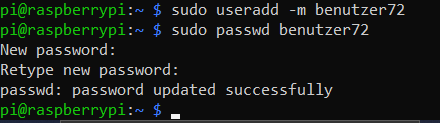
\includegraphics[scale=1]{Bilder/useradd_benutzer72.png}
        \caption{Anlage und Konfiguration des Benutzers \glqq benutzer72\grqq}\label{pic:useradd_72}
    \end{center}
\end{figure}

\begin{figure}[H]
    \begin{center}
        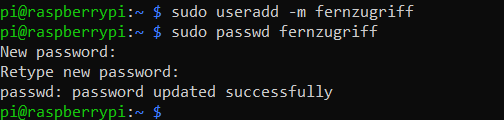
\includegraphics[scale=1]{Bilder/useradd_fernzugriff.png}
        \caption{Anlage und Konfiguration des Benutzers \glqq fernzugriff\grqq}\label{pic:useradd_fernzugriff}
    \end{center}
\end{figure}

\begin{figure}[H]
    \begin{center}
        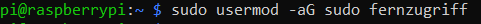
\includegraphics[scale=1]{Bilder/sudo_fernzugriff.png}
        \caption{Benutzer \glqq fernzugriff\grqq{} in die Gruppe sudo aufnehmen}\label{pic:usermod_fernzugriff}
    \end{center}
\end{figure}

\begin{figure}[H]
    \begin{center}
        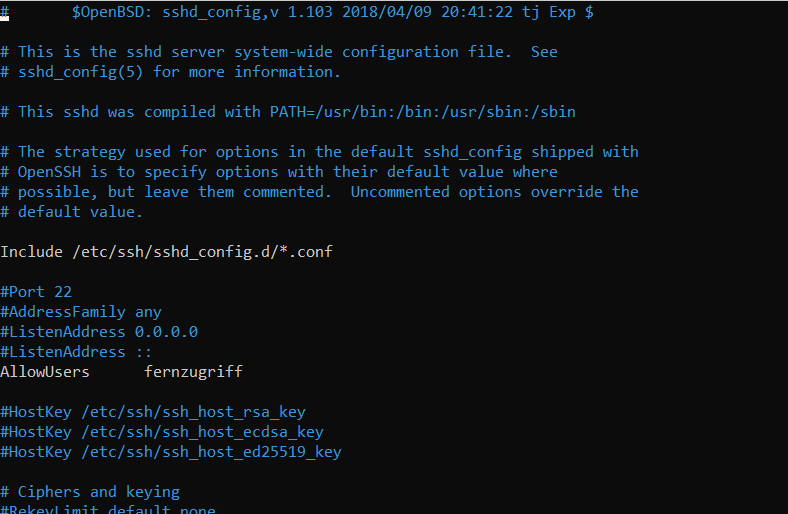
\includegraphics[scale=1]{Bilder/ssh_fernzugriff.png}
        \caption{Benutzer \glqq fernzugriff\grqq{} SSH-Rechte gewähren}\label{pic:ssh_fernzugriff}
    \end{center}
\end{figure}


\subsubsection{Konfiguration Netzwerk}\label{ch:pics_network}
\begin{figure}[H]
    \begin{center}
        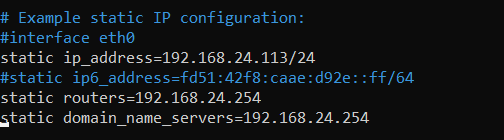
\includegraphics[scale=1]{Bilder/dhcpcdconf.png}
        \caption{Angepasste dhcpcd.conf Datei}\label{pic:dhcpcdconf}
    \end{center}
\end{figure}



\subsubsection{Konfiguration Firewall}\label{ch:pics_firewall}
\begin{figure}[H]
    \begin{center}
        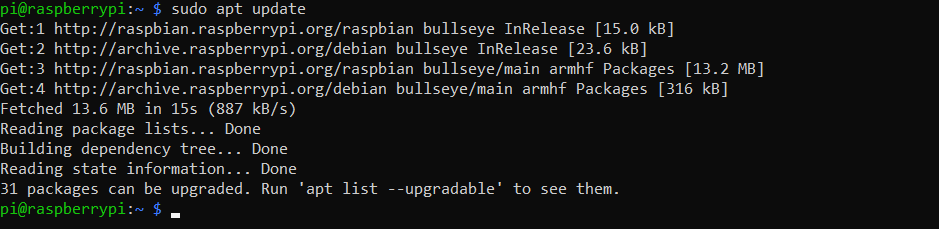
\includegraphics[scale=0.7]{Bilder/update_apt.png}
        \caption{Update APT}\label{pic:udpate_apt}
    \end{center}
\end{figure}

\begin{figure}[H]
    \begin{center}
        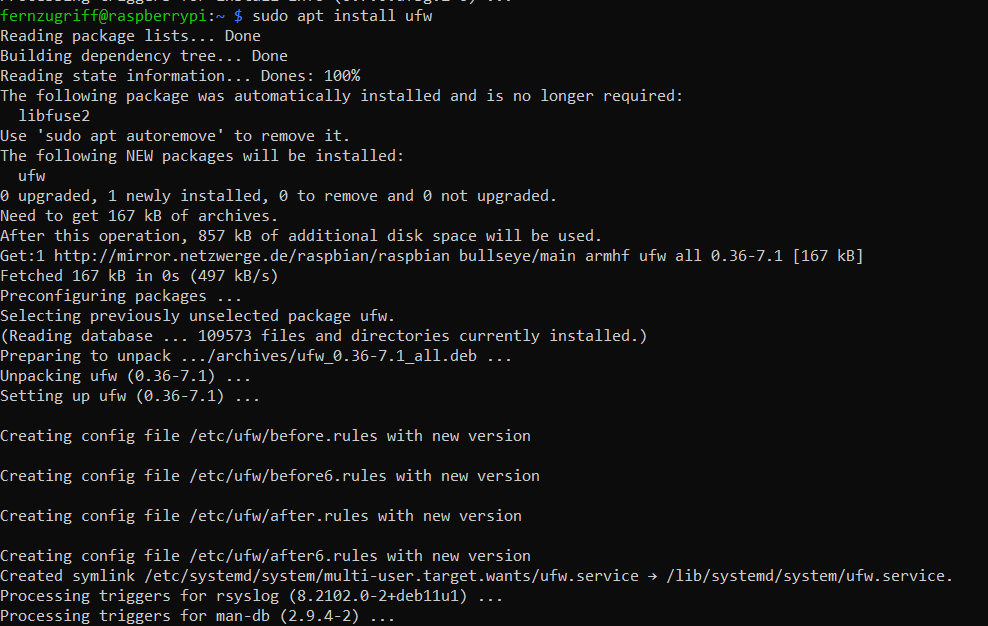
\includegraphics[scale=0.7]{Bilder/install_firewall.png}
        \caption{Installation der UFW Firewall}\label{pic:install_firewall}
    \end{center}
\end{figure}

\begin{figure}[H]
    \begin{center}
        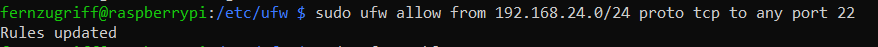
\includegraphics[scale=0.7]{Bilder/allow_ssh_from_network.png}
        \caption{SSH Port für gleiches Netzwerk öffnen}\label{pic:ssh_port_allow}
    \end{center}
\end{figure}

\begin{figure}[H]
    \begin{center}
        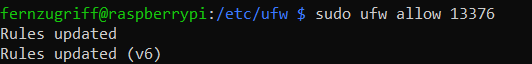
\includegraphics[scale=0.7]{Bilder/ufw_allow_api.png}
        \caption{Port der API für alle Netzwerke freischalten}\label{pic:api_port_allow}
    \end{center}
\end{figure}

\begin{figure}[H]
    \begin{center}
        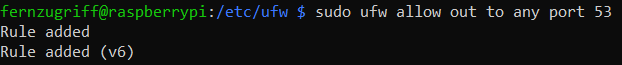
\includegraphics[scale=0.7]{Bilder/ufw_allow_out_dns.png}
        \caption{Ausgehende DNS Anfragen erlauben}\label{pic:dns_allow_out}
    \end{center}
\end{figure}

\begin{figure}[H]
    \begin{center}
        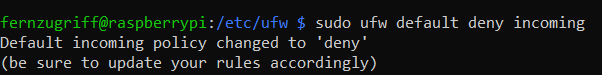
\includegraphics[scale=0.7]{Bilder/ufw_deny_all_incoming.png}
        \caption{Alle eingehenden Pakete ohne Regel verbieten}\label{pic:firewall_deny_default}
    \end{center}
\end{figure}

\subsubsection{Konfiguration Webserver}\label{ch:pics_webserver}
\begin{figure}[H]
    \begin{center}
        
\includegraphics[scale=0.7]{Bilder/apache_simple_start_page.png}
        \caption{Alle eingehenden Pakete ohne Regel verbieten}\label{pic:apache_simple_page}
    \end{center}
\end{figure}





\subsection{Quellen}\label{ch:src}
\subsubsection{Internetquellen}\label{ch:src_internet}
\begin{enumerate}
    \item Ubuntu Wiki: UncomplicatedFirewall. 2022 - Online unter: \newline\url{https://wiki.ubuntu.com/UncomplicatedFirewall} $\left[\text{11.06.2023}\right]$\label{src:ufw}
\end{enumerate}
\begin{small}

\end{small}
\end{document}